\documentclass[11pt,a4paper]{article}
\usepackage[margin=2.3cm]{geometry}
\usepackage{fontspec}
\usepackage{amsmath,amssymb}
\usepackage{booktabs,tabularx,multirow}
\usepackage{graphicx}
\usepackage{float}
\usepackage{caption}
\usepackage{enumitem}
\usepackage{algorithm}
\usepackage{algpseudocode}
\usepackage{tikz}
\usetikzlibrary{arrows.meta,positioning,calc}
\usepackage[hidelinks]{hyperref}
\graphicspath{{../results/}}
\setlist{itemsep=2pt,topsep=4pt}
\newcommand{\code}[1]{\texttt{#1}}
\newcommand{\pct}{\,\%}

\title{Joint Scheduling of Intersection Access\\ and Shared Charging Resources for\\
Delivery Robots in a Dual-Loop Network}
\author{EE6228 course project (topics M02 + M04)}
\date{Pure-software 2-D online simulation}

\begin{document}
\maketitle

\begin{abstract}
Four delivery robots serve two one-way loops that share a single mutually exclusive intersection
and one charging area reachable only through that intersection. We build a deterministic
discrete-event simulator with an independent schedule validator and a browser replay, define a
normalised objective, and compare four heuristics, an offline CP-SAT model that decides order
assignment, order sequence, intersection time slots, charger choice and charging amount jointly, and
an online rolling-horizon variant of it. Over 700 validated runs (10 settings $\times$ 10 seeds
$\times$ 7 strategies), CP-SAT reduces the objective by about 50\pct\ against first-come-first-served
(62\pct\ less tardiness, 28\pct\ shorter makespan) and the online rolling variant by about 37\pct,
while the single-rule baselines stay within a few percent of each other. We also show that a fair
comparison requires the same end-of-horizon battery reserve for every method, and we discuss the
limits of the normalised objective.
\end{abstract}

\section{Case introduction}

Two delivery zones, A and B, are each served by a closed one-way loop. The loops meet at a single
mutually exclusive intersection X, and both zones share one charging area (entrance H, bays C1 and C2)
that can only be reached through X. Four virtual robots work in the network: R1 and R2 serve zone A,
R3 and R4 serve zone B. Pick-up-and-delivery orders arrive over time, each with a release time,
pick-up station, drop-off station, handling times, a due time and a priority.

The two shared resources are coupled. A robot that needs to charge must cross X twice (out and back),
so intersection congestion delays charging; a charging queue in turn shifts every later intersection
request of that robot and of the robots behind it. Batteries make the problem harder still: a robot
may only accept an order if, after completing it, it can still reach a charger without falling below
the safety threshold. The project studies how to coordinate \textbf{task assignment, task order,
intersection time slots, charger choice and charging duration} so that the fleet stays safe and on
time under high load.

\emph{Scope.} Self-designed map and data; robots move along fixed directed routes (no continuous
kinematics or obstacle avoidance); battery, handling and charging are software states. The emphasis
is on scheduling and resource conflicts.

\section{System description}

\subsection{Network}

Each loop is the directed cycle $X \to Z_1 \to Z_2 \to Z_3 \to Z_4 \to W_Z \to X$ for
$Z \in \{A, B\}$ (Figure~\ref{fig:network}). $W_A$ and $W_B$ are the only places where a robot may
wait for the intersection. Every edge that enters X ($W_A \to X$, $W_B \to X$, $H \to X$) is a
\emph{crossing}; X can hold at most one robot, and two consecutive crossings must be separated by a
safety buffer $\beta$ on each side. The charging branch is $X \to H \to C_p \to H \to X$; robots queue
at H, never inside X or an occupied bay, and leave the bay as soon as charging ends.

Because a robot travels around its loop, every lap passes through X: the intersection is not only on
the way to the chargers but on every delivery whose drop-off lies ``behind'' its pick-up, and on every
empty repositioning that wraps around the loop.

\begin{figure}[H]
\centering
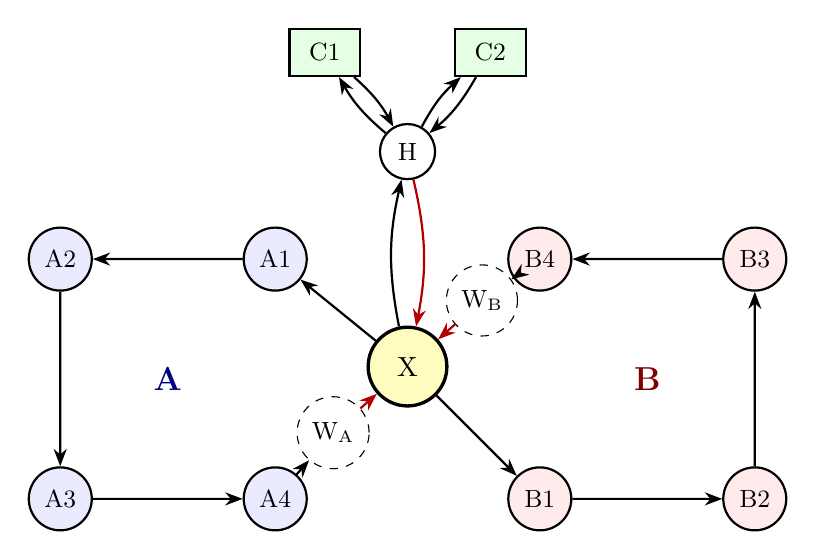
\begin{tikzpicture}[
  st/.style={circle,draw,thick,minimum size=8mm,font=\small},
  wt/.style={circle,draw,dashed,minimum size=7mm,font=\small},
  bay/.style={rectangle,draw,thick,minimum width=9mm,minimum height=6mm,font=\small},
  ed/.style={-{Stealth[length=2.2mm]},thick},
  scale=1.05]
  \node[circle,draw,very thick,fill=yellow!25,minimum size=10mm] (X) at (0,0) {X};
  \node[st,fill=blue!8] (A1) at (-1.6,1.3) {A1};
  \node[st,fill=blue!8] (A2) at (-4.2,1.3) {A2};
  \node[st,fill=blue!8] (A3) at (-4.2,-1.6) {A3};
  \node[st,fill=blue!8] (A4) at (-1.6,-1.6) {A4};
  \node[wt] (WA) at (-0.9,-0.8) {W\textsubscript{A}};
  \node[st,fill=red!8] (B1) at (1.6,-1.6) {B1};
  \node[st,fill=red!8] (B2) at (4.2,-1.6) {B2};
  \node[st,fill=red!8] (B3) at (4.2,1.3) {B3};
  \node[st,fill=red!8] (B4) at (1.6,1.3) {B4};
  \node[wt] (WB) at (0.9,0.8) {W\textsubscript{B}};
  \node[circle,draw,thick,minimum size=7mm,font=\small] (H) at (0,2.6) {H};
  \node[bay,fill=green!10] (C1) at (-1.0,3.8) {C1};
  \node[bay,fill=green!10] (C2) at (1.0,3.8) {C2};
  \draw[ed] (X) -- (A1); \draw[ed] (A1) -- (A2); \draw[ed] (A2) -- (A3);
  \draw[ed] (A3) -- (A4); \draw[ed] (A4) -- (WA); \draw[ed,red!70!black] (WA) -- (X);
  \draw[ed] (X) -- (B1); \draw[ed] (B1) -- (B2); \draw[ed] (B2) -- (B3);
  \draw[ed] (B3) -- (B4); \draw[ed] (B4) -- (WB); \draw[ed,red!70!black] (WB) -- (X);
  \draw[ed] (X) to[bend left=12] (H); \draw[ed,red!70!black] (H) to[bend left=12] (X);
  \draw[ed] (H) to[bend left=10] (C1); \draw[ed] (C1) to[bend left=10] (H);
  \draw[ed] (H) to[bend left=10] (C2); \draw[ed] (C2) to[bend left=10] (H);
  \node[font=\large\bfseries,blue!50!black] at (-2.9,-0.15) {A};
  \node[font=\large\bfseries,red!50!black] at (2.9,-0.15) {B};
\end{tikzpicture}
\caption{Implemented network. Red arrows are crossings into the exclusive intersection X; dashed
nodes are the waiting points in front of X. R1/R2 start at A1, R3/R4 at B1.}
\label{fig:network}
\end{figure}

\subsection{Default parameters}

\begin{table}[H]
\centering\small
\begin{tabular}{lll}
\toprule
Parameter & Base setting & Tested range \\
\midrule
Robots & 4 (2 per loop) & -- \\
Orders & 40 & 20, 40, 60 \\
Initial SOC & uniform 50--100\pct\ per robot (seeded) & -- \\
Safety threshold $S_{\min}$ & 10\pct & 10, 20, 30\pct \\
Ordinary edge & 20\,m, 20\,s, 2\pct & editable lengths \\
Crossing into X & 6\,s & 5--8\,s \\
Safety buffer $\beta$ & 2\,s each side (4\,s between crossings) & 1--4\,s \\
Waiting drain $\rho_w$ & 0.2\pct/min & 0--0.5\pct/min \\
Load / unload & 10--20\,s each, 0.5\pct\ each & -- \\
Charging rate $\rho_c$ & linear, 5\pct/min & 3--8\pct/min \\
Charging bays & 2 & 1, 2 \\
Due time & release + 8--15\,min (tight: 4--8\,min) & -- \\
Priority & 1 (50\pct), 2, 3 & urgent orders 4--5 \\
Zone A share & 50\pct & 1:1, 2:1, 3:1 \\
Urgent orders & 0 & +10\pct, +20\pct\ (due in 3--6\,min) \\
\bottomrule
\end{tabular}
\caption{Default parameters (SOC: battery state of charge in percentage points).}
\end{table}

Orders are released uniformly over $[0, 12n)$ seconds for $n$ orders. The generator is seeded, and
urgent orders and initial SOC come from separate random streams, so adding urgent orders never
changes the base workload of the same seed. All strategies are evaluated on the identical instance.

\subsection{Objective}
\label{sec:objective}

The proposal's objective adds terms with different units: seconds of makespan, seconds of
priority-weighted lateness, seconds of queueing and percentage points of energy. Under load the
lateness term reaches tens of thousands of seconds and would swamp everything else. Each term is
therefore normalised by its value in the FCFS schedule of the same instance, and the four normalised
terms are weighted equally:
\begin{equation}
J = \frac{1}{4}\left(\frac{C_{\max}}{\hat R_C} + \frac{\sum_i p_i T_i}{\hat R_T}
  + \frac{W_{\text{cross}} + W_{\text{charge}}}{\hat R_W} + \frac{E}{\hat R_E}\right),
\label{eq:J}
\end{equation}
\begin{equation}
T_i = \max(0,\, C_i - d_i), \qquad
\hat R_k = \max\!\left(R_k^{\text{FCFS}},\, f_k\right), \qquad
f = (1\,\text{s},\ 60\,\text{s},\ 60\,\text{s},\ 1\pct),
\end{equation}
where $C_{\max}$ is the completion time of the last order, $p_i$ the priority, $C_i$ and $d_i$ the
completion and due time of order $i$, $T_i$ its tardiness, $W$ the total intersection and charger
queueing time and $E$ the total energy consumed. The floors $f_k$ only matter when FCFS has (almost)
no lateness or queueing. FCFS therefore scores $J = 1$ (slightly less when one of its terms is below
its floor), and $J = 0.6$ reads as ``40\pct\ better than FCFS on this weighted balance''. Battery
safety is \emph{not} traded off: falling below the safety threshold is a hard constraint checked by an
independent validator, so $N_{\text{unsafe}} = 0$ in every reported schedule.

\section{Simulator}

The simulator is a dependency-free Python web application (standard-library HTTP server, SVG front
end). Its core is a deterministic discrete-event engine with reservation calendars:
\begin{itemize}
\item \textbf{World and energy model} (\code{simulator.py}, \code{customization.py}): directed edges
  with length, travel time and energy; per-action SOC updates for moving, crossing, waiting, handling
  and charging.
\item \textbf{Reservation calendars}: one for X (with the $2\beta$ gap) and one per bay. A robot
  requesting a resource receives the earliest feasible slot, and the waiting time is recorded as an
  explicit \code{cross\_wait} or \code{charge\_wait} action at an allowed waiting point.
\item \textbf{Independent validator} (\code{validate\_result}): recomputes from the returned action
  log alone the energy of every action, edge legality, route continuity, pickup-before-delivery,
  release times, robot capacity, action overlap per robot, exclusive and buffered resource use
  (derived from the physical trace, not from reservation labels), waiting locations, immediate
  charger departure and SOC bounds. A schedule that fails validation is never returned as a result.
\item \textbf{Replay and analytics} (\code{static/}): the 2-D animation reads only the event log (it
  never recomputes timing), plus a Gantt chart, battery curves, reservation timelines for X/C1/C2, a
  delivery table and a strategy comparison. Tasks, schedule, events, robots and summary export to CSV.
\item \textbf{Command mode}: an external plan (robot, start time, action) can be executed strictly;
  timing, resource and battery conflicts are reported instead of being repaired.
\end{itemize}

\section{Scheduling strategies}

\subsection{Baselines}

\begin{enumerate}
\item \textbf{FCFS} --- orders in release order; each goes to the compatible robot with the earliest
  predicted completion; a robot below 20\pct\ SOC charges before its next order; intersection slots
  are granted in booking order.
\item \textbf{Staged} --- the proposal's ``assign, then reserve the intersection, then charge''
  decomposition. Stage~1 assigns orders by list scheduling on nominal travel times, ignoring X,
  chargers and battery. Stage~2 executes each robot's fixed sequence with intersection reservations.
  Stage~3 inserts a charge only when the next order would otherwise be unsafe.
\item \textbf{Deadline + reservations} --- earliest due date first (priority breaks ties), with the
  resource reservations and energy checks of the full engine.
\item \textbf{Joint greedy} --- evaluates up to eight upcoming orders on both compatible robots,
  including the resulting intersection and charger reservations and charging insertions, and picks
  the candidate with the lowest score
  \[
    \text{score} = C_i + 3\,p_i T_i + 0.5\,W^{\text{new}} + 2\,E^{\text{new}},
  \]
  where $W^{\text{new}}$ and $E^{\text{new}}$ are the queueing and energy added by the candidate.
\end{enumerate}

All automatic strategies keep a battery reserve before accepting an order: the robot must be able to
finish it, reach H and survive the currently booked charger queue plus a conservative allowance for
the other three robots. All heuristics charge to a fixed target of 95\pct.

\subsection{CP-SAT joint optimisation}

The full formulation is in \code{docs/optimizer\_model.md}; this section summarises it. The key
observation is that routes are fixed, so for every pair of consecutive jobs of a robot the travel
time, the energy and the \emph{set of crossings of X} are known in advance. Each robot $k$ gets a
graph $V_k = \{0\} \cup I_k \cup Q_k$ whose vertices are a depot $0$ (its current state), every order
$I_k$ of its loop, and optional charging visits $Q_k$.

\paragraph{Decision variables.}
$x_{ik} \in \{0,1\}$ assigns order $i$ to robot $k$; arc literals $a_{kab} \in \{0,1\}$ choose the
successor of each vertex; $s_i, c_i$ are order start and completion; for each crossing $r$ the entry
time $e_{kr}$ and the wait $w_{kr} \ge 0$ in front of X, with exit $l_{kr} = e_{kr} + \tau_r$; for each
charging visit $q$ a presence literal $y_{kq}$, bay literals $b_{kqp}$, the queue $w^{C}_{kq}$ at H,
charging start $u_{kq}$ and duration $D_{kq}$; the SOC after incoming travel and after service at
every vertex; tardiness $T_i$ and makespan $C_{\max}$.

\paragraph{Constraints.}
\begin{align}
&\textstyle\sum_{k} x_{ik} = 1 \quad \forall i,
  \qquad \textsc{Circuit}\big(\{a_{kab}\}\big) \quad \forall k
  && \text{(assignment)}\\
&a_{kab} = 1 \;\Rightarrow\; s_{b} \ge c_{a}, \qquad s_i \ge r_i
  && \text{(precedence)}\\
&e_{kr} = \text{arrival}_{kr} + w_{kr}, \qquad l_{kr} = e_{kr} + \tau_r
  && \text{(crossing)}\\
&\textsc{NoOverlap}\big(\{[e_{kr},\, l_{kr} + 2\beta)\}_{k,r}\big)
  && \text{(exclusive X)}\\
&u_{kq} = h_{kq} + w^{C}_{kq} + \tau_{Hp}, \qquad
  S^{-}_{kq} = S_{H,kq} - \rho_w w^{C}_{kq} - g_{Hp} \ge S_{\min}
  && \text{(queue at H)}\\
&S^{+}_{kq} = S^{-}_{kq} + \rho_c D_{kq} \le 100, \qquad
  \textstyle\sum_p b_{kqp} = y_{kq}
  && \text{(charging)}\\
&\textsc{NoOverlap}\big(\{[u_{kq},\, u_{kq} + D_{kq}) : b_{kqp} = 1\}\big) \quad \forall p
  && \text{(exclusive bays)}\\
&\mathit{soc}_{\text{out}} = \mathit{soc}_{\text{in}} - \textstyle\sum g_{ab} - \sum g_h
  - \rho_w \sum w \;\ge\; S_{\min}
  && \text{(energy)}\\
&\mathit{soc}_{\text{last}(k)} \ge S_{\min} + G_{k \to H \to p} + \rho_w\, \bar W_{\text{queue}} + \delta
  && \text{(reserve)}
\end{align}
Here $\tau$ and $g$ are edge durations and energies, $g_h$ the handling energy, $h_{kq}$ and
$S_{H,kq}$ the arrival time and SOC at H, $G_{k\to H\to p}$ the energy from the robot's last station
to the cheapest bay, $\bar W_{\text{queue}} = 3\,(95 - S_{\min})/\rho_c$ the heuristics' allowance of
waiting behind three other full recharges, and $\delta = 0.5\pct$ a small margin. Every crossing on every arc and inside every order is an
optional interval that exists only if its arc is chosen; the waits happen at the incoming waiting
point ($W_A$, $W_B$ or H), never inside X. The robot leaves a bay as soon as charging ends, and the
charged amount $\rho_c D_{kq}$ is a decision, unlike the heuristics' fixed 95\pct\ target. The terminal
reserve is the same condition the heuristics enforce before accepting any order. Without the margin
$\delta$ the optimum ended exactly on the boundary and was then rejected by the simulator's check,
which also drains while queueing for X. Tardiness and makespan are linearised with
$T_i = \max(0, c_i - d_i)$ and $C_{\max} = \max_i c_i$ (\code{AddMaxEquality}).

The objective is exactly the normalised $J$ of Eq.~\eqref{eq:J}; its references $\hat R_k$ are
constants computed before the solve, so $J$ stays linear. Time is scaled to milliseconds and SOC to
integer units, with every duration and consumption rounded \emph{up} so that integer-feasible
schedules remain feasible in the exact simulator. The model is warm-started with the joint greedy
schedule (\code{AddHint}).

\paragraph{Decoding.} The solver's choices (sequence, crossing entry times, bay, charging start and
target SOC) are replayed through the simulator's own planner, so times and energy in the returned
schedule come from the simulator, and the result must pass the independent validator. If the decoded
schedule is worse than the warm start or fails validation, the warm start is returned and the
fallback is recorded, so CP-SAT never reports a schedule worse than joint greedy.

\paragraph{Search.} CP-SAT runs with 8 parallel workers. With a single worker the solver did not
improve the warm start on 40-order instances even after about two minutes, while the parallel
portfolio, whose large-neighbourhood-search workers do most of the work, improved it substantially
within the same time. On small instances (4--6 orders) the model reaches proven optimality and
matches the analytical lower bound (unit tests). On realistic sizes the lower bound stays weak, so
the results are good incumbents, not proven optima.

\subsection{Rolling-horizon re-optimisation}

Offline optimisation assumes all orders are known at time 0. The rolling strategy removes that
assumption: an order becomes visible only at its release time (Algorithm~\ref{alg:rolling}).

\begin{algorithm}[H]
\caption{Rolling-horizon CP-SAT}
\label{alg:rolling}
\begin{algorithmic}[1]
\State $t \gets 0$
\While{orders remain}
  \State $\mathcal{K} \gets$ orders released by $t$ and not yet started
  \State $\mathcal{W} \gets$ orders of $\mathcal{K}$, most urgent first, until $\approx 600$\,s of work per loop
  \State $\hat R \gets$ FCFS references of $\mathcal{K}$ continued from the current state \Comment{online normalisation}
  \State plan $\gets$ CP-SAT on $\mathcal{W}$ from the robots' current states, committed X and bay
         reservations fixed (1 worker, deterministic budget $\approx 0.5$\,s, warm start = joint greedy)
  \State commit every job of plan that starts before $t + 60$\,s; freeze its reservations
  \State $t \gets t + 60$\,s
\EndWhile
\end{algorithmic}
\end{algorithm}

Committed actions are never revised. Each window solve requires the last planned job of every robot
to leave the terminal reserve, so that the next window is never left in an energy dead end. Even the
normalisation is online: the references come from an FCFS schedule of only the orders known so far.
An earlier version used full-instance references; the code review showed that this changed
decisions, i.e.\ it leaked future information. The final schedule is scored with the full-instance
$J$ like every other strategy.

\section{Experiments}

\subsection{Setup}

The experiment plan of the proposal is run by \code{experiments.py}. Every configuration uses seeds
1--10; for a given seed all seven strategies (six plus the ablation of Section~\ref{sec:reserve})
receive the identical order list, configuration and seeded initial SOC. The base setting is
40 orders, 2 bays, a 10\pct\ safety threshold, a 1:1 zone split and no urgent orders; one factor is
varied per experiment (Table~\ref{tab:exp}).

\begin{table}[H]
\centering\small
\begin{tabular}{ll}
\toprule
Experiment & Settings \\
\midrule
Algorithm comparison & base \\
Load & 20, 40, 60 orders \\
Charging resources & 1 or 2 bays \\
Zone imbalance & A:B = 1:1, 2:1, 3:1 \\
Safety threshold & 10, 20, 30\pct \\
Dynamic orders & +0, +10, +20\pct\ urgent orders (due 3--6\,min after release, priority 4--5) \\
\bottomrule
\end{tabular}
\caption{Experiment plan.}
\label{tab:exp}
\end{table}

Identical instances that occur in several experiments (the base setting) are solved once, giving
10 distinct settings $\times$ 10 seeds $\times$ 7 strategies $=$ 700 runs. Each run reports $J$, its
four raw terms, the late-order rate, queueing at X and at the chargers, energy, charging sessions and
runtime. Because the seeds differ strongly in difficulty, the tables also give the \emph{paired}
change of $J$ against FCFS on the same instance.

\emph{Compute.} The four heuristics and the rolling strategy are deterministic (rolling solves are
bounded by CP-SAT deterministic time, not wall time), so their schedules do not depend on the
machine; this was checked by reproducing a rolling run bit for bit on two different machines. CP-SAT
is wall-time bounded (120\,s, 8 workers) and therefore hardware dependent; all CP-SAT runs used the
same machine type (Google Colab high-RAM CPU VMs, 8 vCPU Intel Xeon @ 2.20\,GHz, OR-Tools 9.15), one
solve per VM at a time.

\emph{Fairness caveats.} The heuristics and offline CP-SAT know the whole order list in advance (but
never start an order before its release); rolling is the only truly online method. All strategies
end the horizon with the same battery reserve (every robot that executes orders must still be able to
reach a charger behind a full queue; robots without orders never move in any strategy). A first run
of offline CP-SAT without that reserve, kept as the ablation \code{cpsat-nores}, often ended near the
safety floor and frequently skipped charging altogether, which inflated its advantage;
Section~\ref{sec:reserve} quantifies this. The heuristics always charge to 95\pct, whereas CP-SAT
chooses the amount.

\subsection{Algorithm comparison (base setting)}

\begin{table}[H]
\centering\small
\setlength{\tabcolsep}{3.5pt}
\resizebox{\linewidth}{!}{%
\begin{tabular}{lrrrrrrrr}
\toprule
Strategy & $J$ & vs FCFS & Late & Tardiness & Makespan & Charges & Energy & Runtime\textsuperscript{a} \\
 & & mean / median & orders & (s) & (s) & & (\%) & \\
\midrule
FCFS & 1.000 & -- & 52\pct & 26\,028 & 3\,233 & 5.0 & 443 & $<0.1$\,s \\
Staged & 1.067 & $+7$ / $+2$\pct & 51\pct & 27\,264 & 3\,441 & 5.4 & 449 & $<0.1$\,s \\
Deadline + reservations & 1.003 & $0$ / $-4$\pct & 51\pct & 25\,994 & 3\,210 & 4.9 & 438 & $<0.1$\,s \\
Joint greedy & 0.793 & $-21$ / $-23$\pct & 37\pct & 17\,826 & 3\,021 & 3.9 & 386 & 0.3\,s \\
Rolling CP-SAT (online) & 0.636 & $-36$ / $-37$\pct & 37\pct & 15\,651 & 2\,741 & 4.3 & 389 & 49\,s \\
\textbf{CP-SAT} & \textbf{0.468} & $\mathbf{-53}$ / $\mathbf{-54}$\pct & 33\pct & 9\,934 & 2\,317 & 4.2 & 359 & 121\,s \\
CP-SAT w/o reserve (ablation) & 0.349 & $-65$ / $-64$\pct & 23\pct & 5\,032 & 1\,732 & 2.0 & 316 & 121\,s \\
\bottomrule
\end{tabular}}
\caption{Base setting (40 orders, 2 bays, 10\pct\ threshold, 1:1 zones); means over 10 seeds, paired
change of $J$ against FCFS as mean / median. \textsuperscript{a}Measured wall time per instance (the
CP-SAT budget is 120\,s; rolling on a 2-vCPU VM). Full tables: \code{results/results.md}.}
\label{tab:base}
\end{table}

\begin{figure}[H]
\centering
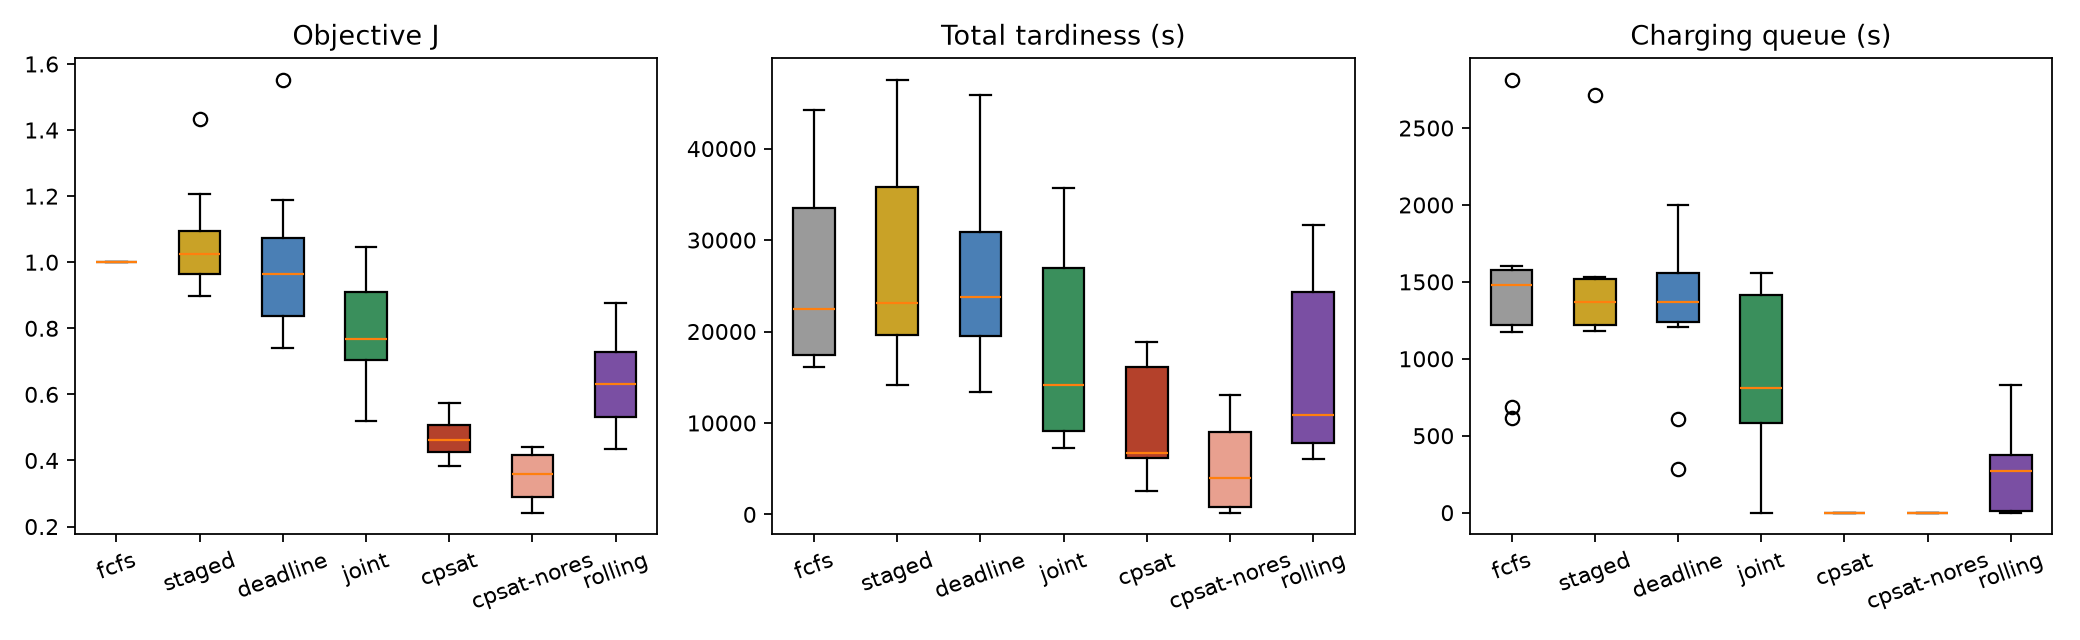
\includegraphics[width=\linewidth]{algorithms.png}
\caption{Base setting, 10 seeds: objective $J$, total tardiness and charger queueing per strategy.}
\label{fig:algorithms}
\end{figure}

All 700 runs produced validated, energy-safe schedules; no strategy failed on any instance. Mean and
median give the same performance tiers, and these hold on most individual seeds
(Figure~\ref{fig:algorithms}): the three single-rule baselines stay within $\pm 7$\pct\ of each other
(their internal order differs: by mean FCFS is marginally ahead of deadline-first, by median
deadline-first is 4\pct\ ahead), joint greedy is about a fifth better, rolling about a third and
offline CP-SAT about a half. Offline CP-SAT never had to fall back to its warm start, but its
optimality gap stays large (base setting: median 58\pct, range 51--70\pct; all 100 instances: median
63\pct, range 18--76\pct): the lower bound of the circuit model is weak, so these are good incumbents,
not proven optima.

\subsection{Sensitivity experiments}

Table~\ref{tab:sens} gives the median paired change of $J$ against FCFS. Means are in
\code{results/results.md}; they differ strongly where near-zero FCFS terms inflate individual runs
(Section~\ref{sec:norm}), e.g.\ at 20 orders staged $+81$\pct\ and deadline $+134$\pct\ by mean against
$+7$\pct\ and $+10$\pct\ by median.

\begin{table}[H]
\centering\small
\begin{tabular}{llrrrrr}
\toprule
Experiment & Setting & Staged & Deadline & Joint & Rolling & CP-SAT \\
\midrule
\multirow{3}{*}{Load} & 20 orders & $+7$ & $+10$ & $-30$ & $-43$ & $-62$ \\
 & 40 orders & $+2$ & $-4$ & $-23$ & $-37$ & $-54$ \\
 & 60 orders & $+8$ & $+10$ & $-16$ & $-18$ & $-47$ \\
\midrule
\multirow{2}{*}{Chargers} & 1 bay & $+45$ & $-1$ & $-20$ & $-28$ & $-60$ \\
 & 2 bays & $+2$ & $-4$ & $-23$ & $-37$ & $-54$ \\
\midrule
\multirow{2}{*}{Imbalance A:B} & 2:1 & $+4$ & $+2$ & $-15$\textsuperscript{b} & $-25$ & $-48$ \\
 & 3:1 & $0$ & $-6$ & $-29$ & $-30$ & $-47$ \\
\midrule
\multirow{2}{*}{Safety threshold} & 20\pct & $+2$ & $+11$ & $-18$ & $-16$ & $-51$ \\
 & 30\pct & $+17$ & $-1$ & $-13$ & $-16$ & $-52$ \\
\midrule
\multirow{2}{*}{Urgent orders} & +10\pct & $+1$ & $-3$ & $-12$ & $-24$ & $-52$ \\
 & +20\pct & $+4$ & $-5$ & $-8$ & $-20$ & $-50$ \\
\bottomrule
\end{tabular}
\caption{Median paired change of $J$ against FCFS (\%), 10 seeds per cell. \textsuperscript{b}Mean
$+19$\pct: one seed scores $J = 3.7$ although joint beats FCFS on makespan, lateness and energy there
(Section~\ref{sec:norm}).}
\label{tab:sens}
\end{table}

\begin{figure}[H]
\centering
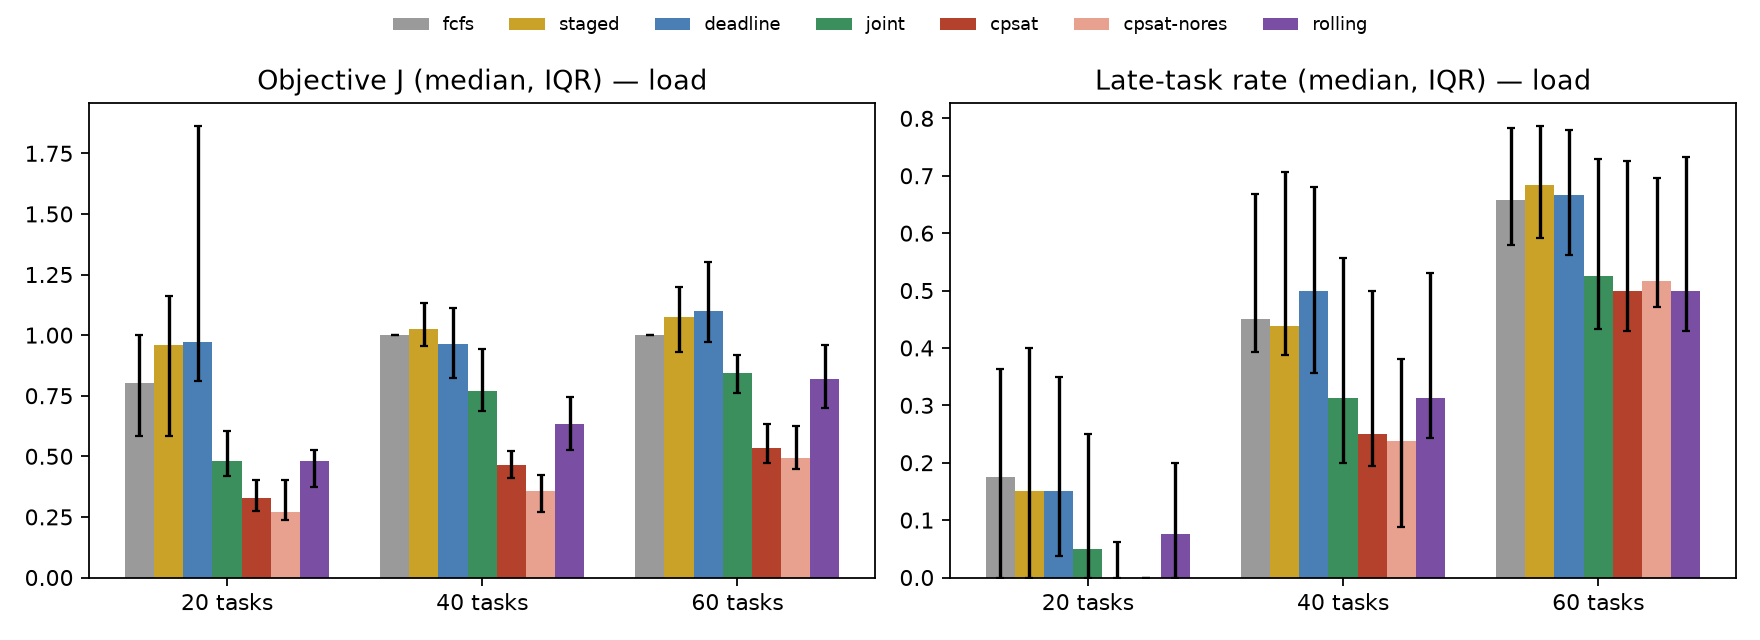
\includegraphics[width=\linewidth]{load.png}
\caption{Load experiment: median $J$ and late-order rate with interquartile range.}
\label{fig:load}
\end{figure}

\begin{itemize}
\item \textbf{Load.} Every method degrades as orders are added, but the gap to FCFS shrinks for the
  heuristics and for rolling ($-43$\pct\ $\to$ $-18$\pct) while CP-SAT keeps $-47$\pct\ to $-62$\pct\
  (Figure~\ref{fig:load}). At 60 orders every method is late on more than half the orders (late rate
  54--69\pct); the fleet is over capacity, and charging (7--10 sessions of up to 17\,min) is the
  binding resource.
\item \textbf{One charging bay.} FCFS's charger queue grows from 1\,437\,s to 4\,001\,s, and the staged
  baseline collapses ($+45$\pct): it decides charging last, so robots arrive at the single bay
  together. Joint greedy and CP-SAT, which decide charging together with the orders, hold their
  advantage; CP-SAT improves most ($-60$\pct).
\item \textbf{Zone imbalance.} With more work on loop A, makespan grows for all methods because R1/R2
  become the bottleneck. The tiers are unchanged (CP-SAT, then rolling and joint greedy, then the
  single-rule baselines), although within the baseline tier deadline-first falls slightly behind FCFS
  by median at 2:1 ($+2$\pct).
\item \textbf{Safety threshold.} A higher threshold forces more charging for everyone. CP-SAT is
  insensitive ($-51$\pct\ / $-52$\pct), while rolling falls back to the level of joint greedy
  ($-16$\pct): each of its windows must end with a full reserve, which with a 20--30\pct\ threshold
  forces early charging that an offline view would avoid.
\item \textbf{Urgent orders.} Short-deadline, high-priority orders hurt every method; offline CP-SAT
  keeps about $-50$\pct, rolling $-20$\pct\ to $-24$\pct. Deadline-first ordering, the obvious rule for
  urgent work, gains only 3--5\pct.
\end{itemize}

\begin{figure}[H]
\centering
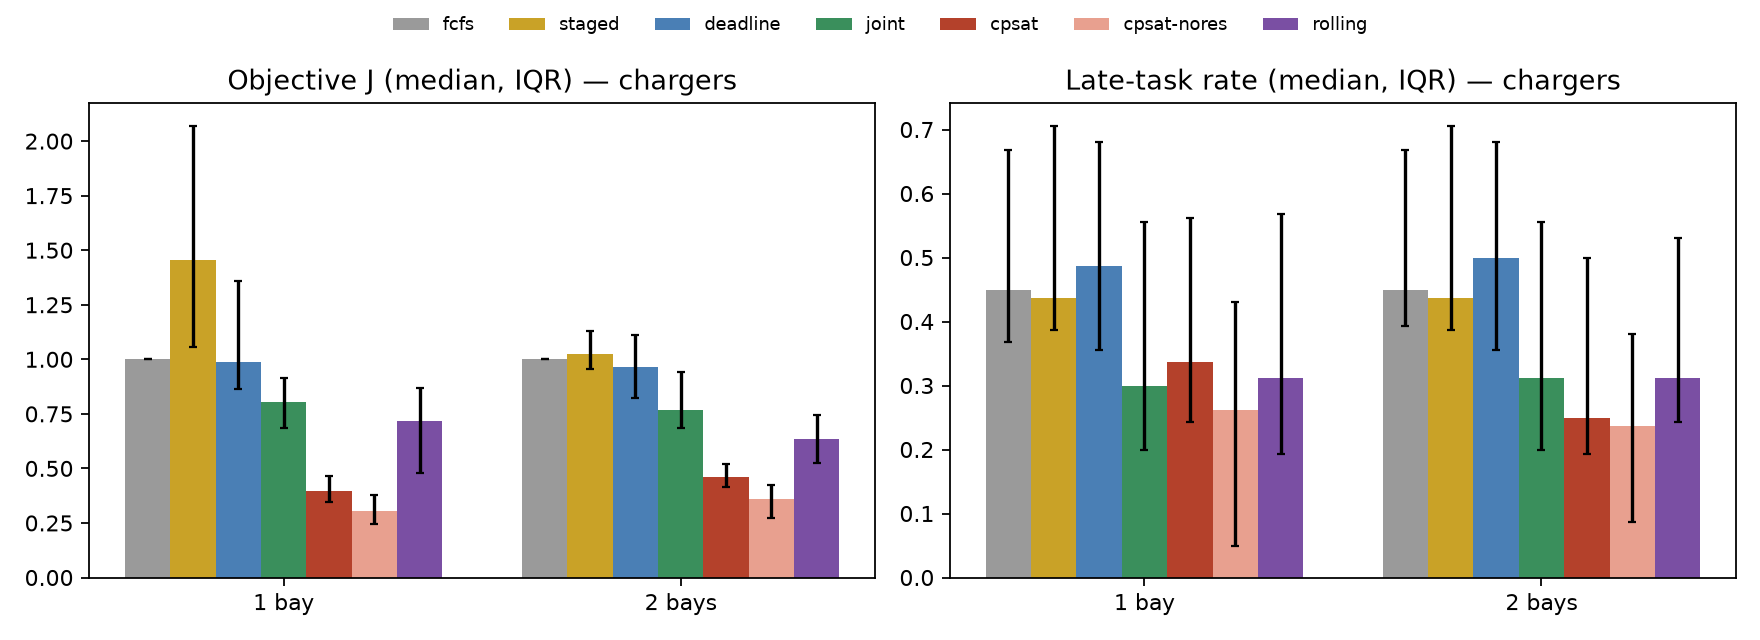
\includegraphics[width=0.92\linewidth]{chargers.png}\\[2pt]
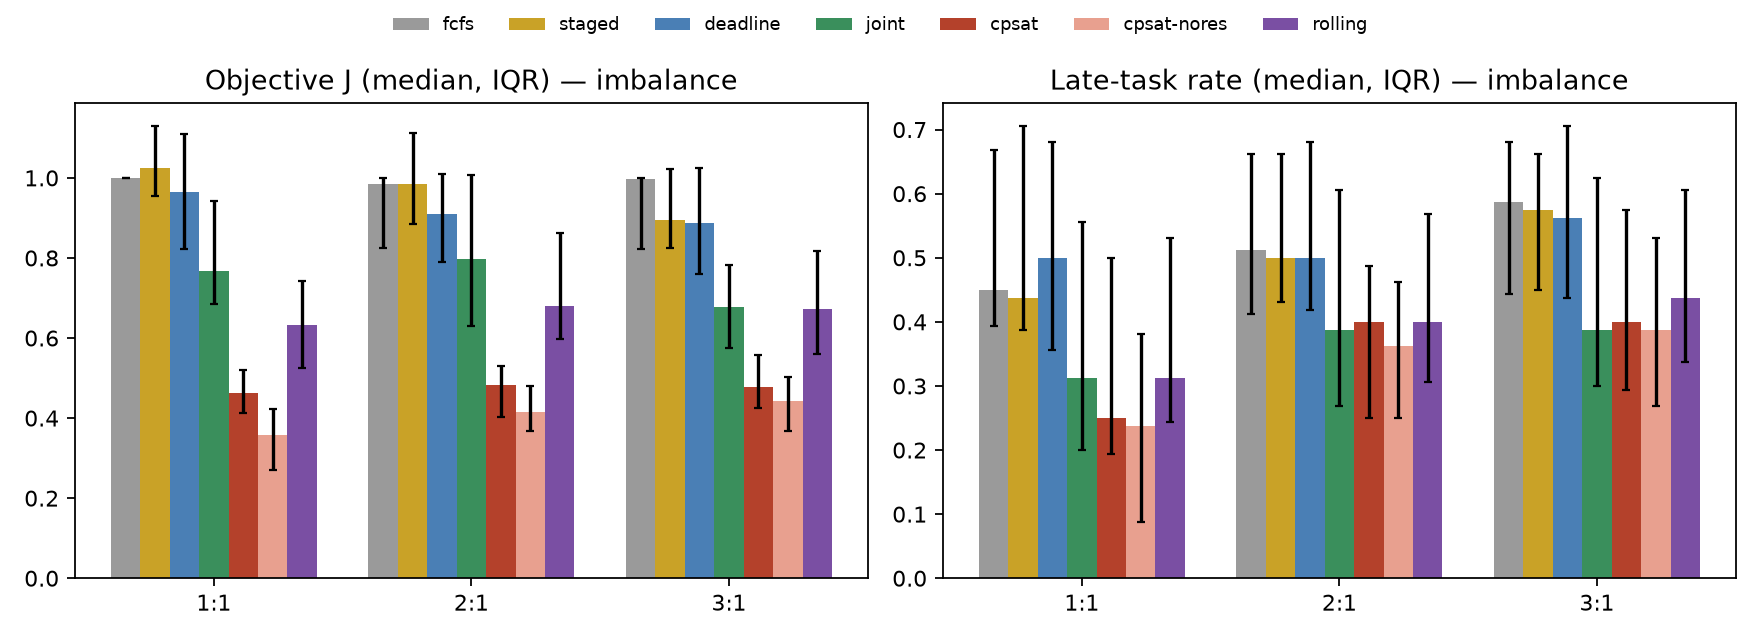
\includegraphics[width=0.92\linewidth]{imbalance.png}
\caption{Charger and zone-imbalance experiments (median, IQR).}
\end{figure}

\begin{figure}[H]
\centering
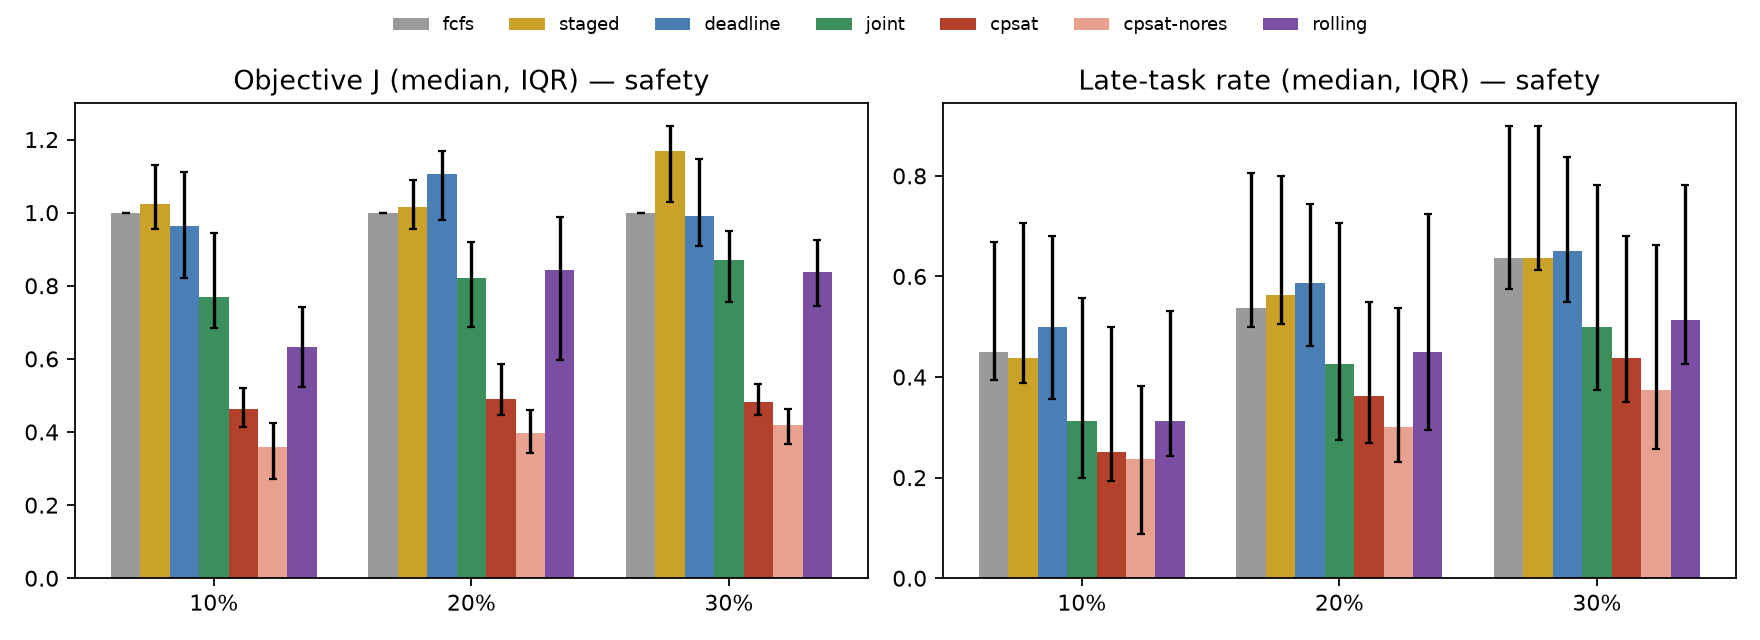
\includegraphics[width=0.92\linewidth]{safety.png}\\[2pt]
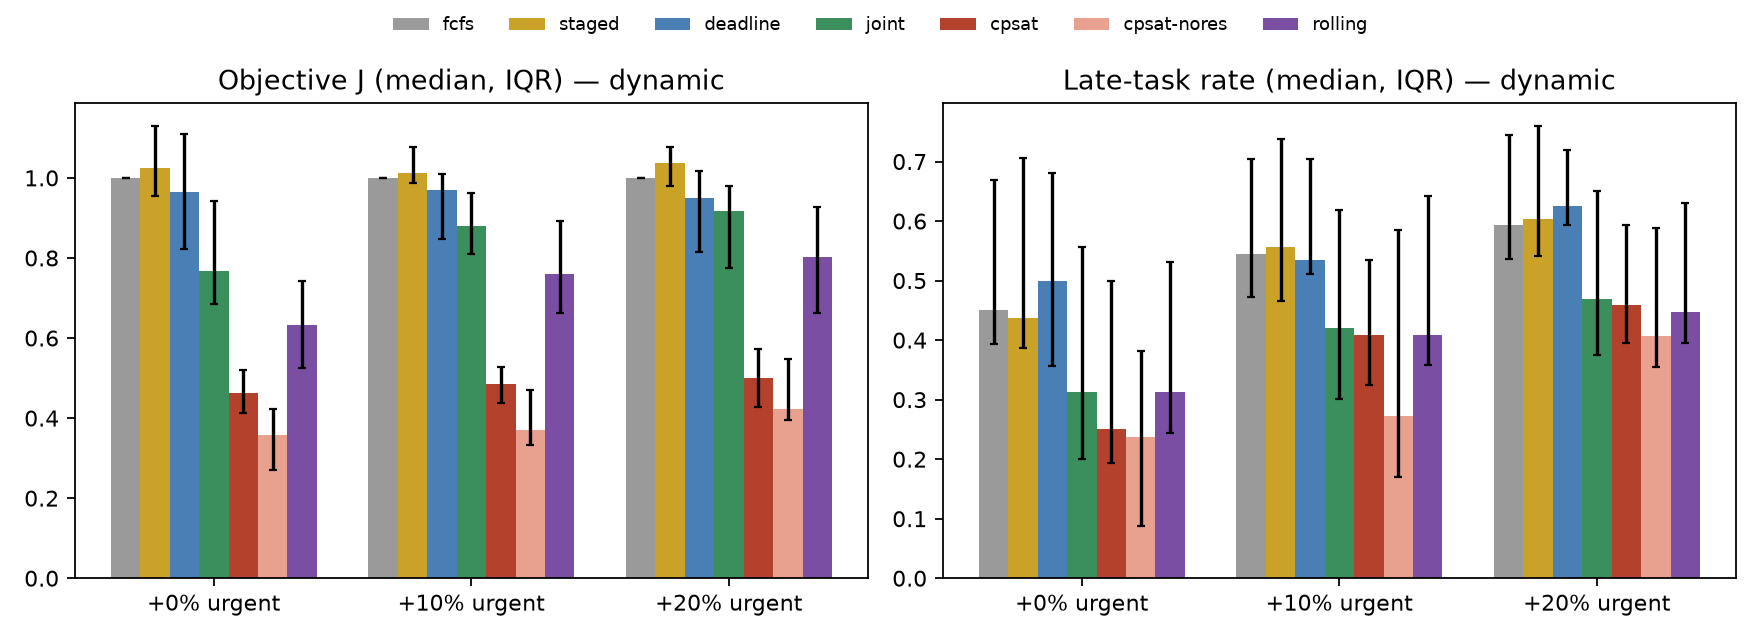
\includegraphics[width=0.92\linewidth]{dynamic.png}
\caption{Safety-threshold and urgent-order experiments (median, IQR).}
\end{figure}

\section{Discussion}

\subsection{Where does the improvement come from?}

Decomposing $J$ into its four normalised terms (base setting, mean contribution; FCFS contributes
0.25 per term) shows that the methods improve in different ways (Table~\ref{tab:terms}).

\begin{table}[H]
\centering\small
\begin{tabular}{lrrrrrr}
\toprule
Strategy & $C_{\max}$ & Tardiness & Queueing & Energy & $J$ & $J'$\textsuperscript{c} \\
\midrule
FCFS & 0.250 & 0.250 & 0.250 & 0.250 & 1.00 & 1.00 \\
Joint greedy & 0.233 & 0.182 & 0.160 & 0.218 & 0.79 & 0.84 \\
Rolling & 0.211 & 0.157 & 0.048 & 0.219 & 0.64 & 0.78 \\
CP-SAT & 0.178 & 0.088 & 0.000 & 0.202 & 0.47 & 0.62 \\
CP-SAT w/o reserve & 0.132 & 0.039 & 0.000 & 0.178 & 0.35 & 0.47 \\
\bottomrule
\end{tabular}
\caption{Mean contribution of each normalised term to $J$ (base setting).
\textsuperscript{c}$J' = (C_{\max} + \text{tardiness} + \text{energy})/0.75$, i.e.\ $J$ re-weighted
over the three terms other than queueing.}
\label{tab:terms}
\end{table}

Both CP-SAT methods \emph{almost eliminate queueing} (CP-SAT: 5.6\,s on average, all of it on one
seed; the heuristics: 23--37\,s at X plus 0.9--1.5 thousand seconds at the chargers). The robots still
wait, but as powered-down standby at their last station before departing, not in front of X or at H.
In the model, standby is free while queueing drains the battery and counts in $J$, so the optimiser
delays departures until the resource is free; the heuristics instead book a slot and drive to the
waiting point. This is legitimate within the model, but about half of CP-SAT's gain in $J$ is the
queueing term. Without that term the tiers are unchanged ($J'$ in Table~\ref{tab:terms}) and CP-SAT
is still the clear winner: it cuts total tardiness by 62\pct\ and the makespan by 28\pct\ against FCFS
(44\pct\ and 23\pct\ against joint greedy).

A plausible main source of the tardiness reduction is charging: CP-SAT charges about as often as
joint greedy (4.2 vs 3.9 sessions) but chooses \emph{how much} to charge and when, whereas the
heuristics always charge to 95\pct, at 5\pct/min up to 17 minutes per session, often in the middle of a
busy period. CP-SAT also changes assignment, order and departure times at the same time, so the
experiments do not isolate this effect; a CP-SAT run with a fixed 95\pct\ target would be the
controlled test.

\subsection{The end-of-horizon reserve}
\label{sec:reserve}

The first CP-SAT experiments did not require any battery left after the last order. The optimiser
then often ended near the safety threshold and skipped charging whenever the initial charge
sufficed: on every 20-order instance it never charged, and on 40 orders it charged half as often as
the heuristics (2.0 vs 3.9--5.4 sessions). The heuristics always keep enough charge to reach a bay
behind a full queue. Imposing the same reserve on CP-SAT raised its $J$ from 0.349 to 0.468 at
40 orders but hardly mattered at 60 orders ($-51$\pct\ vs $-47$\pct\ median), where robots must charge
anyway. About a fifth of offline CP-SAT's apparent advantage at moderate load (12 of 65 percentage
points) was therefore an end-of-horizon effect. Any offline comparison against continuous-operation
policies needs an explicit terminal condition.

A second, smaller lesson: the optimiser placed the terminal SOC exactly on the reserve boundary, and
the simulator's reserve check, which also drains while queueing for X, rejected many of those plans,
which then fell back to the warm start (during development, 32 of 115 result rows of a partial run,
some instances counted in several experiments; those rows were discarded). After the margin $\delta =
0.5$\pct\ was added, none of the 100 final instances fell back. Exact model/simulator agreement matters
most precisely where an optimiser pushes against a constraint.

\subsection{The normalised objective}
\label{sec:norm}

Normalising by FCFS achieved its purpose: without it, priority-weighted tardiness (tens of thousands
of seconds) would dominate the other terms by two orders of magnitude, and the four terms contribute
comparably. The price is instability on instances where an FCFS term is close to zero. On one 2:1
instance FCFS queued for only 18\,s, so the queueing term was divided by its 60\,s floor, and joint
greedy's 735\,s of queueing alone added $0.25 \times 735/60 \approx 3.06$ to its $J$ (total 3.7),
although joint beat FCFS on makespan, lateness and energy. The same effect produces means above 1 for
staged and deadline at 20 orders (medians 0.96--0.97). Medians and paired comparisons are therefore
reported throughout. A more robust choice would normalise by fixed, instance-independent scales (e.g.\
the mean over the whole experiment) or by the instance's median over all strategies.

\subsection{Online versus offline}

Rolling is the only method that does not know future orders, yet in the base setting it beats every
heuristic that does (median $-37$\pct\ vs $-23$\pct\ for joint greedy), and it stays 8--14 percentage
points ahead of joint greedy with 20 orders, one bay, 2:1 imbalance and urgent orders. Its weaknesses
are the ones expected of a receding horizon: with a 20--30\pct\ safety threshold its per-window reserve
forces early charging, and at 60 orders or 3:1 imbalance its short look-ahead cannot plan around the
bottleneck, so it is only level with joint greedy (and slightly behind it at a 20\pct\ threshold). Its
re-plans are bounded by deterministic solver work (about 1\,s each on a 2-vCPU machine, 49\,s for a
full 40-order day), so it would run in real time. With the same OR-Tools version, one worker and a
wall-clock cap that does not bind, its schedules are bit-identical across machines (checked on two
machines); runtimes of course differ.

\subsection{Limitations}

\begin{itemize}
\item CP-SAT results depend on hardware (wall-time budget); all were produced on one machine type.
\item Optimality gaps are large; better lower bounds (e.g.\ a relaxation per loop) would be needed to
  claim near-optimality.
\item The heuristics see all future orders, which favours them against rolling, but not against
  offline CP-SAT.
\item The charging model is linear, the network has a single intersection, and robots move on fixed
  routes without kinematics.
\end{itemize}

\section{Conclusion}

A simulator for two delivery loops that share one intersection and one charging area was built, with
an independent validator, a browser replay and an experiment pipeline that compares six strategies
(plus one ablation) on identical, seeded instances. Over 700 validated runs:
\begin{enumerate}
\item \textbf{Deciding orders, intersection slots and charging jointly pays off.} In the base setting
  the single-rule baselines (FCFS, deadline-first, staged) stay within a few percent of each other,
  the joint greedy heuristic gains about 20\pct\ and CP-SAT, which optimises all decisions in one
  model, about 50\pct\ in $J$ (62\pct\ less tardiness, 28\pct\ shorter makespan than FCFS). Across all
  sensitivity settings CP-SAT stays at $-47$\pct\ to $-62$\pct\ (median), joint greedy varies between
  $-8$\pct\ and $-30$\pct, and the staged baseline can be much worse than FCFS ($+45$\pct\ with one
  bay).
\item \textbf{Charging is the bottleneck.} Under load the chargers, not the intersection, limit the
  fleet: for every heuristic the mean queueing at X stays under a minute per run, while charger queues
  reach thousands of seconds. Choosing how much and when to charge is the most plausible source of
  CP-SAT's lower lateness (not isolated experimentally), and separating the charging decision from
  assignment (the staged baseline) is worst with a single bay.
\item \textbf{Online re-optimisation is practical.} Rolling CP-SAT, without knowledge of future
  orders, beats all heuristics at moderate load with about a second per re-plan; under heavy load or a
  high safety threshold it is only level with the joint greedy heuristic.
\item \textbf{Fair comparison needs care.} Requiring the same end-of-horizon battery reserve changed
  the CP-SAT result substantially ($J$: 0.35 $\to$ 0.47), and the normalised objective must be read
  with medians because near-zero reference terms can dominate it.
\end{enumerate}

\end{document}
